\section{Introduction}
\label{sec:intro}
\dan{TODO}
\begin{figure}
    \centering
        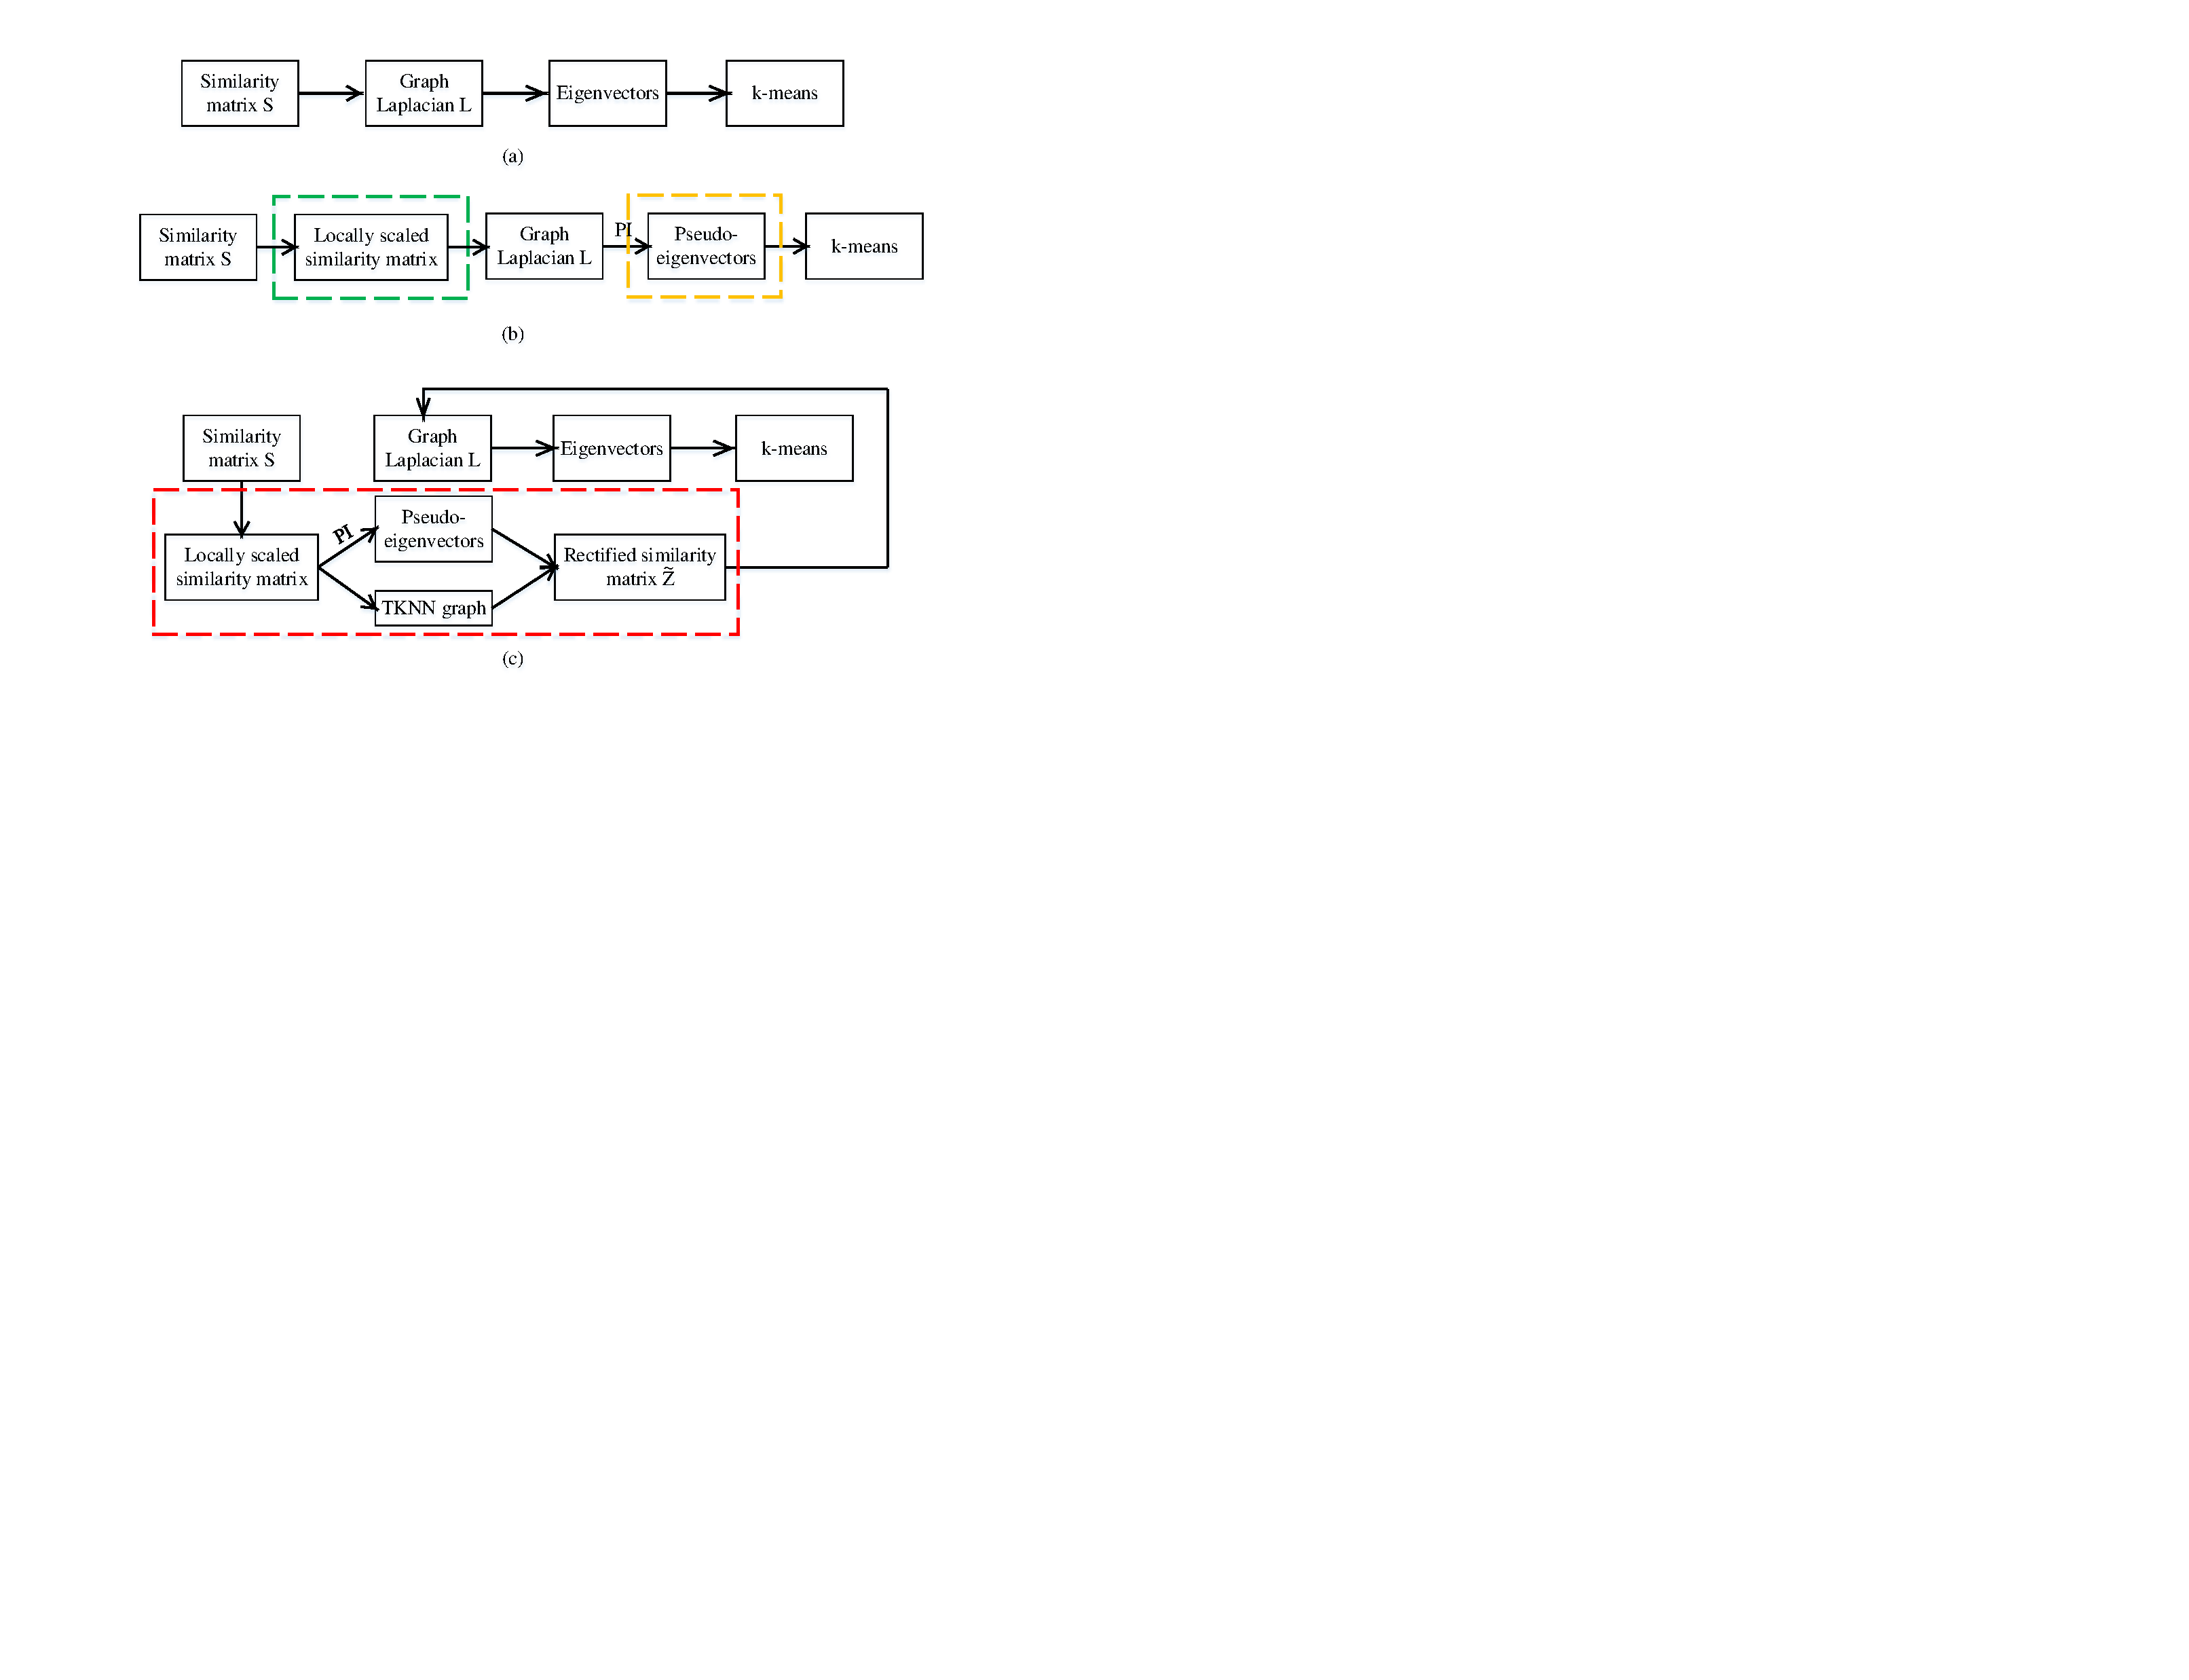
\includegraphics[width = 1.09\linewidth]{flow_graph3.pdf}
        \caption{The key steps of (a) basic spectral clustering; (b) with local scaling and PI; (c) ROSC}
        \label{figure:flow_graph}
\end{figure}


\comment{
For example, for a 2-cluster partition $V=V_1 \cup (V \backslash V_1)$, 
the \emph{normalized cut} is defined as
\begin{equation}
\label{eq:ncut}
Ncut(V_1, V\backslash V_1) = \sum_{i\in V_1,j\in V\backslash V_1} S_{ij}[\frac{1}{a(V_1)} + \frac{1}{a(V\backslash V_1)}]
\end{equation}
where $a(V_1) = \sum_{i\in V_1, j\in V}S_{ij}$.
Minimizing the normalized cut was proposed in~\cite{shi2000normalized} and
the optimization problem is NP-hard.
It has been shown that cuts based on the eigenvector corresponding to the second largest eigenvalue of the normalized graph Laplacian
$D^{-1}(D-S)$
give a guaranteed approximation to the optimal cuts~\cite{chung1997spectral,shi2000normalized},
where $D$ is a diagonal matrix with $D_{ii} = \sum_jS_{ij}$.
It is easy to further extend the normalized cut criterion to the case of $k$ clusters,
and cuts based on the largest $k$ eigenvectors will give a guaranteed approximation.
From this viewpoint, spectral clustering is closed related with the spectral analysis to a matrix.
However, since the object cluster membership is hard,
mapping from these eigenvectors to the discrete cluster membership is required.
}

\comment{
Clustering fundamentally serves as an analysis tool in data mining and machine learning,
and spectral clustering is one important type.
Some basic clustering methods, such as $k$-means and EM clustering~\cite{dempster1977maximum}, 
explicitly or implicitly pre-assume that data should fit specific distributions.
%which assumes data follows Gaussian distribution.
Obviously, when data is complex, these methods tend to fail.
%especially those which contain non-Gaussian distributed clusters.
In contrast, spectral clustering may work well on such data.
Instead of making assumptions on the data distribution,
it translates clustering into a graph partition problem,
which aims to achieve strong intra-cluster relations and weak inter-cluster relations between objects.
Objects are clustered by a spectral analysis on the normalized graph Laplacian,
which has been theoretically proved~\cite{chung1997spectral,spielmat1996spectral}.
}

\comment{
\begin{figure}
    \centering
        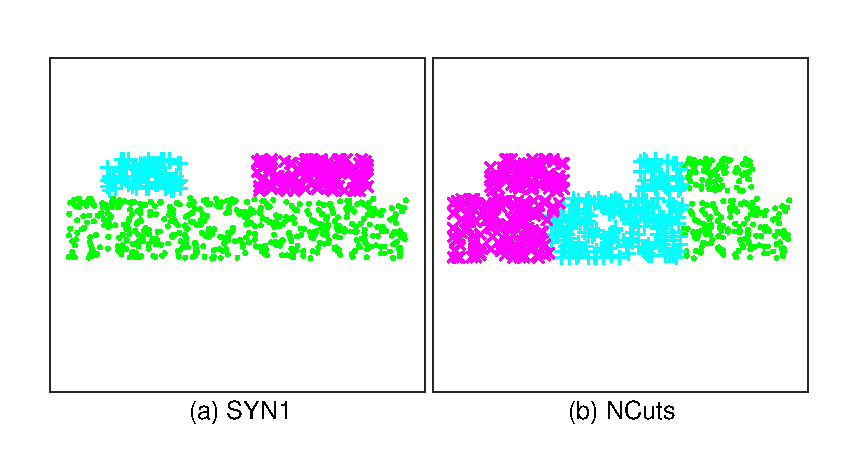
\includegraphics[width = \linewidth]{figure/syn1_intro.eps}
        \caption{An toy example}
        \label{figure:SYN1_intro}
\end{figure}
}

%%%%%%%%%% Ben: I masked the results of SYN1 because we are thinking of removing it.
\begin{figure}
    \centering
        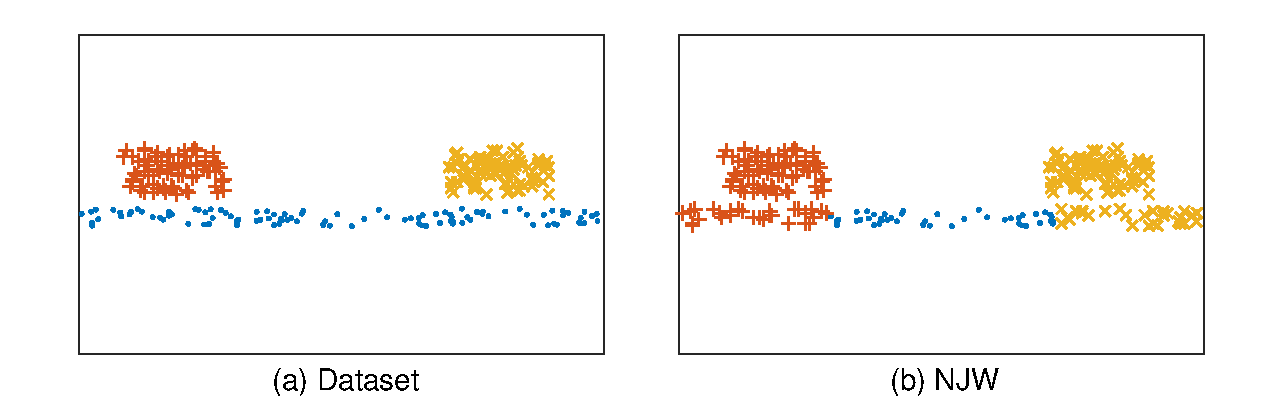
\includegraphics[width = \linewidth]{figure/example_intro.eps}
        \caption{(a) A multi-scale dataset, (b) clustering by NJW}
        \label{figure:syn1}
\end{figure}

Despite the successes of spectral clustering, previous works have
pointed out that spectral methods
can be adversely affected by the presence of 
\emph{multi-scale data}~\cite{zelnik2004self,nadler2006fundamental},
which is defined as data whose object clusters are of various sizes and densities.
As an illustrative example, 
Figure~\ref{figure:syn1}(a) shows a dataset of three clusters: 
two dense rectangular clusters on top of a narrow sparse stripe cluster.
Figure~\ref{figure:syn1}(b) shows the result of applying the standard spectral clustering method NJW
to the dataset. We see that the stripe cluster is segmented into three parts, two of which are
incorrectly merged with the rectangular clusters. 
The objective of this paper is to address the multi-scale data issue in spectral clustering. 
In particular, we review existing methods for handling multi-scale data, provide insight into how
the issue can be addressed, and put forward our algorithm called ROSC which outperforms existing 
methods in clustering multi-scale data.

There are two general approaches to address the multi-scale data problem: one on scaling the similarity matrix 
$S$ and another on applying the power iteration technique to obtain pseudo-eigenvectors that contain rich cluster separation
information.

Recall that spectral clustering methods model data objects as a graph and
perform clustering by graph partitioning.
The similarity matrix $S$ should therefore capture objects' local neighborhood information. 
A common choice of such a similarity function is the
Gaussian kernel:
$\sij = \exp \left(-\frac{||\bmx_i-\bmx_j||^2}{2\sigma^2}\right)$,
where $\bm x$ (boldface) denotes a feature vector of an object $x$, 
%$||\cdot||$ denotes the standard Euclidean distance
and $\sigma$ is a global scaling parameter.
A major difficulty in using the Gaussian function to cluster multi-scale data lies in the choice of
$\sigma$. 
If $\sigma$ is set small, then $\sij$ will become small.  Objects in a sparse cluster (which are 
relatively distant among themselves compared with objects in a dense cluster) will likely be
judged as dissimilar leading to partitioning of the cluster. On the other hand, if $\sigma$ is set large,
$\sij$ will be large. Hence,
nearby dense clusters could be judged similar to each other and are inadvertently merged. 

To tackle this problem, the ZP method~\cite{zelnik2004self} applies {\it local scaling} and modifies the Gaussian similarity
to $\sij = \exp\left (-\frac{||\bmx_i-\bmx_j||^2}{\sigma_i\sigma_j}\right)$.
Here, $\sigma_i$ (and likewise for $\sigma_j$) is a local scaling parameter for object $x_i$.
It is defined as the distance between $x_i$ and its $l$-th nearest neighbor for some 
empirically determined value $l$.
If $x_i$ is located in a sparse cluster, then $\sigma_i$ will be large.
This boosts the similarity of $x_i$ and its neighboring objects and thus avoids the splitting of 
sparse clusters. 
Also, if $x_i$ is located in a dense cluster, $\sigma_i$ will be small.
Objects will have to be very close to be considered neighbors.
This avoids the merging of nearby dense clusters. 

Previous studies~\cite{alpert1995spectral,ye2016fuse} have suggested that employing more eigenvectors beyond the $k$ smallest ones
can help capture more cluster separation information and thus improve spectral clustering in handling multi-scale data.
A {\it power iteration} (PI) method~\cite{saad2011numerical} was put forward as an efficient method for computing the
dominant eigenvector of a matrix. 
It is observed in~\cite{lin2010power} that one can
{\it truncate} the iteration process to obtain an 
intermediate \pev\ $\bmv_t$.
It is shown that $\bmv_t$ represents a weighted linear combination of all the eigenvectors and is thus
a very effective replacement of the $k$ smallest eigenvectors typically used in a standard spectral
clustering process. 
Figure ~\ref{figure:flow_graph}(b) shows how the local-scaling method (green box) and the power iteration method (yellow box)
are integrated into the basic spectral clustering method. 

In this paper we take a different approach to tackle the multi-scale data problem. 
The core idea is to construct an $n \times n$  coefficient matrix $Z$ such that the entry $\zij$\footnote{Given a matrix $M$, 
%unless otherwise specified, 
we use a pair of subscripts to specify an entry of $M$.} reflects how well 
an object $x_i$  characterizes another object $x_j$. 
Our objective is to derive such a $Z$ with  ``grouping effect'': 
if two objects $x_i$ and $x_j$ are highly correlated (and thus should be put into the same cluster), 
then their corresponding coefficient vectors 
$\bmz_i$ and $\bmz_j$ given in $Z$ are similar.
The interesting question we address is how to find such a $Z$.

The main feature of our algorithm ROSC is illustrated by the red box shown in Figure ~\ref{figure:flow_graph}(c). 
Instead of using PI to obtain low dimensional embeddings of the objects as input to $k$-means
(yellow box in Figure ~\ref{figure:flow_graph}(b)),
ROSC uses the embeddings to construct the matrix $Z$ (upper path in the red box).
We note that two objects that belong to the same cluster could be located at distant far ends of a cluster,
their high correlation is therefore not expressed properly by a distance-based similarity matrix $S$.
To capture the high correlation between distant objects in the same cluster,
we propose to use a transitive $K$ nearest neighbor (TKNN) graph (lower path in the red box). 
Two objects $x_i$ and $x_j$ are connected by an edge in the TKNN graph
if there is a sequence of objects $<x_i, \ldots, x_j>$ such that adjacent objects in the sequence 
are mutual $K$ nearest neighbors of each other. 
We use the TKNN graph to regularize the matrix $Z$ so that it possesses the desired grouping effect.
The matrix $Z$ is then fed to the pipeline of spectral clustering, taking the role of $S$.

%To tackle the problem,
%researchers mainly focus on two aspects.
%First, construct a more effective similarity matrix.
%The Gaussian kernel is based on the feature distance between objects, 
%however, in the case of clusters with multiple densities,
%the average distance between objects in the sparse cluster is larger than in the dense cluster.
%Therefore, 
%the average similarity between objects in the sparse cluster is smaller than in the dense cluster,
%leading to the sparse cluster being more likely to be partitioned.
%A representative method in this kind is 
%the self-tuning spectral clustering method ZP.
%Instead of using the global scaling parameter, 
%ZP considers the local statistics information for each object
%and calculates $S_{ij} = exp(-\frac{||\bmx_i-\bmx_j||^2}{\sigma_i\sigma_j})$,
%where $\sigma_i,\sigma_j$ denote the local scaling parameters for objects $\bmx_i,\bmx_j$ respectively.
%$\sigma_i$ is set to be the distance between $\bmx_i$ and its $l$-th neighbor,
%where $l$ is set empirically.
%By considering the local density, ZP can increase the similarity between objects in the sparse cluster.
%However, when clusters are of uniform density but different sizes,
%objects will have similar local scales and ZP will fail. 
%Further, the miscalculation on $\sigma_i$ can also lead to the poor clustering performance.

\comment{
Second, employ more eigenvectors.
%The standard spectral clustering methods use only $k$ eigenvectors.
%(or the $k$ largest eigenvectors of the graph similarity matrix).
%However, it is not unlikely that the $k$-th eigenvector corresponds to some particularly salient noise in the data,
%while the $k$+1-th eigenvector contains good cluster indicators and then it will be missed totally~\cite{lin2010power}.
It has been pointed out that when dealing with clusters of different scales, 
standard spectral clustering using only $k$ eigenvectors may fail~\cite{nadler2006fundamental,ye2016fuse}.
Therefore, some works propose to use more eigenvectors to derive more cluster-separation information
based on power iteration, which provides a way to fuse information in all eigenvectors (will be introduced in the next section).
However, more eigenvectors also bring the redundancy and noise problem, 
which further bring negative effects.
%Recently, power-iteration based methods have attracted great attention.
%the full spectral clustering method FUSE was proposed to
%fuse the useful cluster-separation information in all the eigenvectors, but 
%it neglects the noise reduction.
Finally,
we emphasize that methods of both kinds 
are not mutually independent.
Some approaches use more eigenvectors based on a locally scaled similarity matrix.
The difference is that 
the former focuses more on the similarity matrix construction 
while the latter highlights more on the usage of eigenvectors based on a given similarity matrix.
}

\comment{
On the other hand,
more eigenvectors can indeed bring more cluster-separation information, but in the meantime, 
more redundancy and more noise,
which further arouses the redundancy and noise reduction problem.
Existing methods attempt to address these problems, 
but no one can be widely applied.
For example, the self-tuning spectral clustering method ZP~\cite{zelnik2004self},
which introduces local scaling, may fail 
when large clusters have comparable densities with small clusters~\cite{nadler2006fundamental};
the full spectral clustering method FUSE~\cite{ye2016fuse}, 
which adopts \emph{independent component analysis} (ICA) to 
reduce redundancy, neglects noise reduction in their case.
To investigate the robustness of these methods, 
we first conduct a group of experiments on two multi-scale datasets as shown in Fig.~\ref{figure:syn1}(a) and~\ref{figure:syn2}(a) respectively. 
}

\comment{
The first dataset consists of 
three uniformly distributed clusters with 500, 80 and 120 objects respectively.
Since the largest rectangular cluster is of large length,
the two-end objects in the cluster are far away from each other,
i.e., they are less similar. 
Further, the closeness between the two small clusters and the large cluster increases more difficulty in clustering.
The second dataset
is composed of five clusters:
two Gaussian distributed with 100 objects each,
two uniformly distributed with 150 and 200 objects respectively 
and an annular cluster with 100 objects.
The annular cluster is close to the other clusters and it is hard to be identified.
Fig.~\ref{figure:syn1} and~\ref{figure:syn2} also show the clustering results for ZP and FUSE.
We observe that ZP performs well on SYN2 but poorly on SYN1 
while FUSE works better on SYN1 but fails on SYN2.
We further notice that ROSC, our proposed method in this paper,
achieves favorable results on both datasets.
From Fig.~\ref{figure:syn1},
ROSC can identify the three clusters with some errors in the small clusters
while FUSE separates the large cluster into two clusters.
From Fig.~\ref{figure:syn2}, ROSC performs well in identifying the annular cluster
while ZP correctly finds Gaussian distributed and uniformly distributed clusters
with misclassification on some objects in the annular cluster.
Obviously, ROSC is more robust than ZP and FUSE.
}

\comment{
Although existing methods attempt to improve spectral clustering on multi-scale data,
we notice that they are unstable.
The instability originates from the fact that none of them settles the problem from the origin.
The effect of spectral clustering depends on the quality of the similarity matrix.
Suppose a block diagonal matrix is given, in which each block corresponds to one cluster,
spectral clustering can definitely perform well because there exist only intra-cluster similarities but no inter-cluster similarities.
Some approaches aim to construct a locally scaled similarity matrix,
but the difficulty in estimating the local scales may 
result in inaccurate similarities which fail in reflecting the true similarities between objects.
Further, they lack a scheme to rectify these inaccurate similarities. 
Different from all the existing methods,
this paper attempts to improve spectral clustering from the origin of the problem. 
Given a similarity matrix, we aim to derive a new matrix which can better reflect the true similarities between objects.
To achieve such goal,
the new matrix should inherit the accurate similarities in the original matrix
and further rectify the inaccurate ones.
The rectified matrix will lead to more robust spectral clustering, as shown in Fig.~\ref{figure:syn1}(b) and~\ref{figure:syn2}(b).
}

\comment{
While these two bottlenecks have attracted great attention,
most of the proposed methods are dedicated to only one aspect~\cite{yan2009fast,chen2011large,zelnik2004self,li2007noise}.
Recently, Ye et al.~\cite{ye2016fuse} put forward a novel method FUSE 
to address both the two problems simultaneously.
Since eigen-decomposition requires high time complexity, it employs \emph{power iteration},
in which eigenvector calculation is replaced by a small number of matrix-vector multiplications,
to derive a set of pseudo-eigenvectors.
The derived pseudo-eigenvectors are fused by all the eigenvectors, 
which contain all the cluster-separation information.
Then it adopts \emph{Independent Component Analysis} (ICA)~\cite{learned2003ica, bohm2008outlier} to rotate these vectors 
and get statistically independent ones.
These pseudo-eigenvectors are then regarded as feature vectors, 
to which k-means would be applied to derive the final clustering result.
FUSE achieves both effectiveness and efficiency, 
however, there still remain some problems. 
First, the derived pseudo-eigenvectors may be redundant and noise corrupted. 
Despite rotation by ICA reducing redundancy, the noise still remains, which weakens the effectiveness.
Second, a self-adaptive greedy strategy is developed to search for directions towards the optimal solution, however,
it might still be trapped in the local optimum.
Third, the time complexity of FUSE relies on
the maximal rank considered by the low-rank decomposition algorithms for pair-wise mutual information estimation in ICA. 
When the rank is as close as $n$, FUSE will run slowly. 
To this end, spectral clustering deserves further exploration from both perspectives of effectiveness and efficiency.
}

Our main contributions are:

\noindent$\bullet$
We proposed a heterogeneous graph convolution algorithm that is capable of capturing edge information.

\noindent$\bullet$
\dan{don't know}

\noindent$\bullet$
We conduct extensive experiments %using synthetic and real datasets 
to evaluate the performance of HINGCN
against $9$ other classification methods. 
Our results show that HINGCN performs very well against the competitors. 
In particular, it is very robust in that it consistently performs well over all the datasets tested. 
Also, it outperforms others by wide margins for datasets that are highly multi-scale. 

The rest of the paper is organized as follows.
%In Section~\ref{sec:preliminary} we give more details of spectral clustering and briefly 
%describe the power iteration method.
Section~\ref{sec:related} mentions related works on heterogeneous graph neural networks, graph embedding and described several semi-supervised classification algorithms.
Section~\ref{sec:algorithm} presents the HINGCN algorithm.
Section~\ref{sec:exp} describes the experiments and presents experimental results.
Finally, Section~\ref{sec:conclusion} concludes the paper.



%\noindent{\small$\bullet$}
%We propose a transitive $K$ nearest neighbor (TKNN) graph.
%In the graph,
%objects in the same cluster but far away in the feature space can be connected
%while objects in different clusters but close to each other can be disconnected.
%
%\noindent{\small$\bullet$}
%We put forward a robust spectral clustering method ROSC on multi-scale data.
%Based on power iteration, ROSC fuses more cluster-separation information in more eigenvectors
%and reduces the redundancy and noise contained.
%%and it integrates the noise reduction with matrix rectification.
%It further applies the TKNN graph to rectify the raw similarity matrix 
%and derives a more effective one,
%leading to a more robust spectral clustering.
%
%\noindent{\small$\bullet$}
%We conduct extensive experiments to
%prove the robustness of ROSC.
%We compare ROSC with state-of-the-art methods on both synthetic and real datasets
%with respect to three clustering measures.
%All the experimental results show that ROSC is indeed a robust spectral clustering method.

\comment{
Recently, in machine learning and computer vision areas, 
%data can be viewed as points drawn from multiple low-dimensional subspaces, with each subspace corresponding to one category or class.
subspace segmentation has been well studied,
which aims to segment (cluster) high-dimensional objects into the low-dimensional subspaces where they are drawn from.
A number of methods have been proposed, such as LRR~\cite{liu2010robust}, LSR~\cite{lu2012robust}, etc.
In these methods, given a set of data vectors $\mathcal{X} = [\bm{x}_1, \bm{x}_2,...,\bm{x}_n]$ (each column is an object) in $\mathbb{R}^d$, 
each object is represented by 
a linear combination of the basis in a dictionary $A = [\bm{a}_1,\bm{a}_2,...\bm{a}_m]$:
\begin{equation}
\nonumber
X = AZ,
\end{equation}
where $Z$ is a coefficient matrix.
Considering the case that data vectors are corrupted by noise, 
a more robust model is thus modified as 
\begin{equation}
\nonumber
X = AZ + E,
\end{equation}
where $E$ is utilized to capture noise.
Subject to the constraint, different optimization objectives on $Z$ (and $E$) are adopted by different methods,
and they desire to derive a low-dimensional mapping $Z$ which can reflect the true subspace structure in the original data.

In this paper, we aim to improve spectral clustering from both effectiveness and efficiency.
Similar to FUSE, we first use power iteration to derive a set of pseudo-eigenvectors 
which inherit all the cluster-separation information in all the eigenvectors.
Then we resort to the subspace segmentation model to purify the pseudo-eigenvectors.

To be continued.
}










